\documentclass[journal,12pt,twocolumn]{IEEEtran}
\usepackage[utf8]{inputenc}
\usepackage{amssymb,amsmath,mathtools} 
\usepackage{amsfonts}  
\usepackage{graphicx}  
\usepackage{times}
\usepackage{gensymb}
\graphicspath{{images/}}
\DeclareGraphicsExtensions{.pdf,.eps,.ps,.png,.jpg,.jpeg}
\newcommand{\C}{\circ}
\title{\textbf{AI1110 Assignment 1}
\author{AI21BTECH11001 }}
\date{March 2022}

\begin{document}

\maketitle
\begin{center}
{ICSE Grade 10 2014 paper}\end{center}

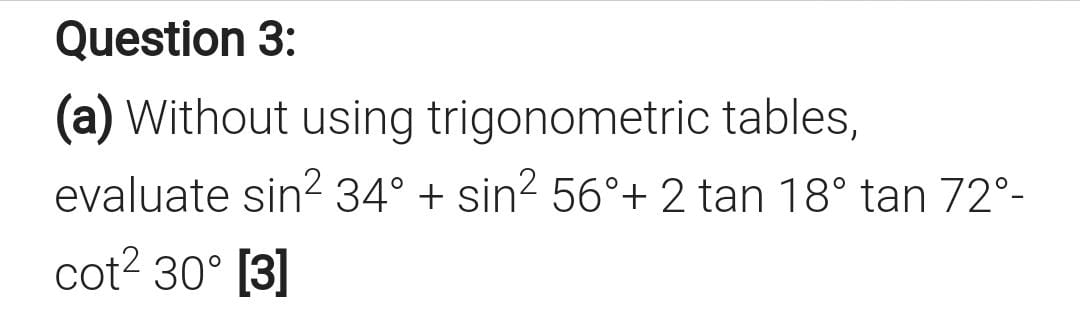
\includegraphics[scale=0.22]{main.jpeg}

\textbf{Solution:}
\begin{align}
= \sin^2 34\degree+ \sin^2 56\degree+2\tan 18\degree \tan 72\degree - \cot^2 30\degree
\end{align}
\begin{align}
 &\sin^2 56\degree = \sin^2 (90\degree - 34\degree)\\
  \implies&\sin^2 56\degree =\cos^2 (56\degree)
  \end{align}
  \begin{align}
  &2\tan18\degree\tan72\degree = 2\tan18\degree\tan(90 - 18)\degree\\
  \implies &2\tan18\degree\tan72\degree = 2\tan18\degree\cot18\degree
 \end{align}
 \begin{align}
= \sin^2 34\degree +\cos^2 34\degree +2\tan18\degree \cot18\degree -\cot^2 30\degree
\end{align}
 \begin{align}
&= 1 + 2\times \tan18\degree \times\frac{1}{tan18\degree} - (\sqrt{3})^2\\
&= 1 + 2 - 3
 = 0\end{align}

\end{document}
